\documentclass[a4paper]{article}

\usepackage{fullpage} % Package to use full page
\usepackage{parskip} % Package to tweak paragraph skipping
\usepackage{tikz} % Package for drawing
\usepackage{amsmath}
\usepackage{mathrsfs}
\usepackage{hyperref}
\usepackage{listings}
\usepackage{xcolor}
\usepackage{float}
\usepackage{indentfirst}
\usepackage{pdflscape}





\usepackage[margin=1in]{geometry}



\restylefloat{table}
\lstset { %
    language=C++,
    backgroundcolor=\color{black!5}, % set backgroundcolor
    basicstyle=\footnotesize,% basic font setting
}
\usepackage{fancyvrb}
\usepackage{booktabs}
%%%%%%%%%%%%%%%%%%%%%%%%%%%%%%%%%%%%%%%%%%%%%%%%%%%%%%%%%%%%%%%%%%%%%%%%%%%%%%%%%%
%				Begining
%%%%%%%%%%%%%%%%%%%%%%%%%%%%%%%%%%%%%%%%%%%%%%%%%%%%%%%%%%%%%%%%%%%%%%%%%%%%%%%%%%

\linespread{1.6}

\begin{document}
%\maketitle

\begin{center}
\thispagestyle{empty} % Na stronie tytu�owej nie chcemy numeru strony

\includegraphics[width=4cm, height=4cm]{logo_uj.png} % Ta komenda umieszcza na stronie logo UJ

{\large JAGIELLONIAN UNIVERSITY

Faculty of Mathematics and Computer Science

} \vfill

{\huge Line Follower - example simulation of performance based on mathematical model of robot}
\vfill

{\large KAROL FARBANIEC}



{\large 
CRACOW, 2017} \pagebreak
\end{center}



\tableofcontents

\newpage
\section{Introduction - problem description}

Linefollowing robot mision is to pass the race as fast as possible. The trajectory of movement is in general closed curve on plane parallel to earth surface.
Mathematical model and simulation of an object response under influence of physical phenomenas should help us understand the meaning of given parameters 
in reference to performance of robot. In few examples this kind of modelling will let us to do inverted process i.e. calculating the
values of parameters for given project specification. Model of a system will be simplified with omitting some phenomenas which do not have big influence
on passing race. The most improratant processes in physical world in reference to movement of a robot will be linked with mathematical statements 
resulting from laws and theorems of Physics.

Modelling and simulation should let us find answers for questions like:

\begin{itemize}
\item How to choose motors for robot in reference to radius and friction of wheel?
\item What are the natural frequencies of mechanical model?
\item What is the influence of track defects on response of model?
\item Which information could by possibly lost in ADC and DAC conversion based on light sensor model?
\item How to protect the information in signal from aliasing effect?
\end{itemize}

%
%
%
%
\newpage

\section{Solution of a problem}

%
%
%
% opis matematyczny i zastosowane wzory
%

Model of static friction between wheel and route surface has been build by applying laws and theorems of Physics, especially Mechanics:

\begin{figure}[!ht]
\begin{center}
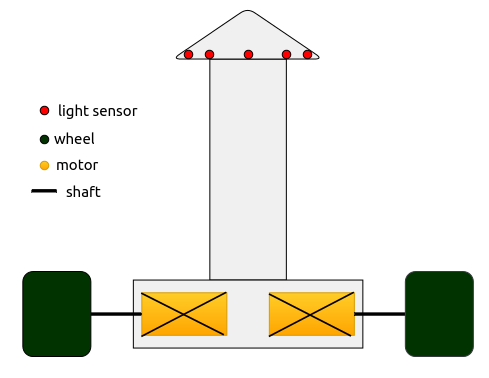
\includegraphics[width=12cm]{1.png}
\caption{Simplified scheme of a robot}
\end{center}
\end{figure}

\begin{figure}[!ht]
\begin{center}
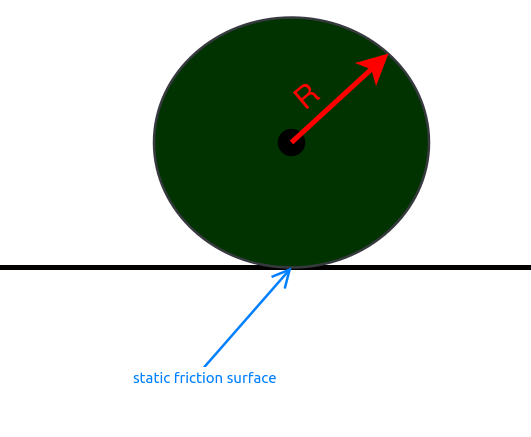
\includegraphics[width=8cm]{2.png}
\caption{Friction surface}
\end{center}
\end{figure}
\newpage

While passing the boundary value of static friction force the wheels will start to slide.
The desinger of robot obejctive due to achieving good control of movement is to find
relationship between geometrical and material parameters of wheels and friction process.

Starting torque of motor should be enough high to start the slide of wheel, but later
controlled in a proper manner. \newline
Let's denote $ \mu$ as a static friction coefficient. newline
Static friction force is proportional to load generated by robot. $T = \mu N $, where
$N$ - load of robot.



Force on tread wheel is given by equation:

\begin{equation}\label{eq:1}
%x\floor n \floor \star h\floor n\floor = y\floor n\floor
F = \frac{M_n}{R}
\end{equation}

Assuming that the force generated by motors should be higher than static friction resistance
final torque statement is:

\begin{equation}\label{eq:2}
M_n > R \mu N
\end{equation}
\newpage

Mass-spring-damper system model. Let's assume viscous damping between mass elements and 
apply Newtons laws of movement for given system.


\begin{figure}[!ht]
\begin{center}
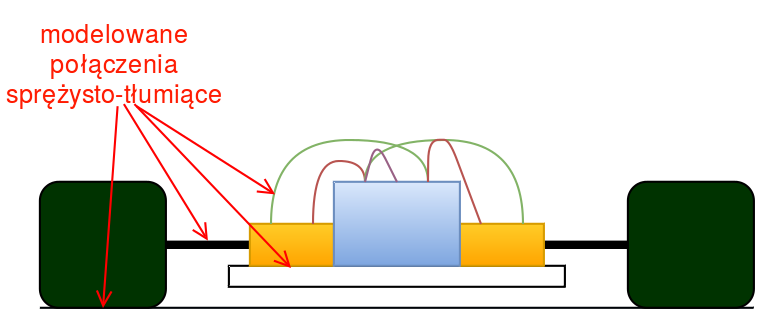
\includegraphics[width=12cm]{3.png}
\caption{mass-spring-damper in reference to physical system}
\end{center}
\end{figure}
\newpage
Model of robot is symetrical, so we will calculate only one half of it.
Discretize mass elements and model the connections between masses: \newline


\begin{figure}[!ht]
\begin{center}
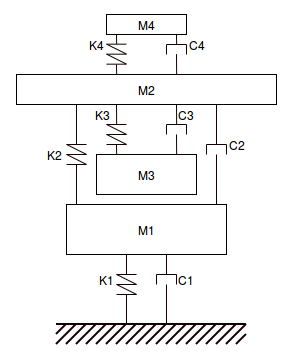
\includegraphics[width=8cm]{4.png}
\caption{mass-spring-damper model}
\end{center}
\end{figure}

Element 1 - wheel of robot \newline
Element 2 - drive and controler \newline
Element 3 - the support element with light sensors \newline
Element 4 - cables and trunk lines\newline
%
%
%
%
% BUDOWA MODELU W PRZESTRZENI STAN�W
% 
% 
% 
% 
System of dynamic equations: \newline
\begin{center}
 $
F_{1} - m_{1} \ddot{x_{1}} - c_{1}\dot{x_1} - k_{1}x_{1} - (x_{1}-x_{2})k_{2} - (\dot{x_{1}} - \dot{x_{2}})c_{2} = 0
$ 
\end{center}
\begin{center}
$
F_{2} - m_{2} \ddot{x_{2}} - c_{2}( \dot{x_{2}} - \dot{x_{1}} ) - k_{2}(x_{2}-x_{1}) - k_{3}(x_{2}-x{3}) - c_{3}(\dot{x_{2}} - \dot{x_{3}}) - k_{4}(x_{2} - x_{4}) - c_{4}(\dot{x_{2}} - \dot{x_{4}}) = 0
$

\end{center}
\begin{center}
$
F_{3} - m_{3}\ddot{ x_{3} } - k_{3}(x_{3} - x_{2}) - c_{3}( \dot{x_{3}} - \dot{x_{2}} ) = 0
$
\end{center}
\begin{center}
$
F_{4} - m_{4}\ddot{x_4} - k_{4}(x_{4}-x_{2}) - c_{4}(\dot{x_{4}} - \dot{x_{2}}) = 0
$
\end{center}

State variables: \newline
$h_{1} = x_{1} ,$ $ h_{2} = \dot{x_{1}},$ $  h_{3} = x_{2} ,$ $  h_{4} = \dot{x_{2}},$ $  h_{5} = x_{3} ,$ $  h_{6} = \dot{x_{3}},$ $  h_{7} = x_{4} ,$ $  h_{8} = \dot{x_{4}}
$ \newline
State-space model of system: \newline
%\[ 
%  \begin{matrix}
%  \begin{pmatrix}x & y\end{pmatrix}\\\mbox{}
%  \end{matrix}
%  \begin{pmatrix} a & b \\ c & d \end{pmatrix} 
%  \begin{pmatrix} x \\ y \end{pmatrix}
%\]

\begin{landscape}
$
  \begin{pmatrix} \dot{h_{1}} \\ \dot{h_{2}} \\ \dot{h_{3}} \\ \dot{h_{4}} \\ \dot{h_{5}} \\ \dot{h_{6}} \\ \dot{h_{7}} \\ \dot{h_{8}} \end{pmatrix} = 
  \begin{pmatrix} {0}&{1}&{0}&{0}&{0}&{0}&{0}&{0} \\
  
  {-(k_{1}+k_{2})}&{-(c_{1} + c_{2})}&{k_{2}}&{c_{2}}&{0}&{0}&{0}&{0} \\
  
  {0}&{0}&{0}&{1}&{0}&{0}&{0}&{0} \\
  
  {k_{2}}&{c_{2}}&{-(k_{2}+ k_{3}+ k_{4})}&{-(c_{2}+ c_{3}+ c_{4})}&{k_{3}}&{c_{3}}&{k_{4}}&{c_{4}} \\
 
  {0}&{0}&{0}&{0}&{0}&{1}&{0}&{0} \\
  
  {0}&{0}&{k_{3}}&{c_{3}}&{-k_{3}}&{-c_{3}}&{0}&{0} \\
  
  {0}&{0}&{0}&{0}&{0}&{0}&{0}&{1} \\
  
  {0}&{0}&{k_{4}}&{c_{4}}&{-k_{4}}&{-c_{4}}&{0}&{0}  
  
  \end{pmatrix}
  \begin{pmatrix} {h_{1}} \\ {h_{2}} \\{h_{3}} \\{h_{4}} \\{h_{5}} \\{h_{6}} \\{h_{7}} \\{h_{8}} \\ \end{pmatrix}
  +
  \begin{pmatrix} {0} & {0} & {0} & {0} \\
  {\frac{1}{m_{1}}} & {0} & {0} & {0} \\
  {0} & {0} & {0} & {0} \\
  {0} & {\frac{1}{m_{2}}} & {0} & {0} \\
  {0} & {0} & {0} & {0} \\
  {0} & {0} & {\frac{1}{m_{3}}} & {0} \\
  {0} & {0} & {0} & {0} \\
  {0} & {0} & {0} & {\frac{1}{m_{4}}} 
  \end{pmatrix}
  \begin{pmatrix}
   F_{1} \\ F_{2} \\ F_{3} \\ F_{4}
  \end{pmatrix}
$ 
\newline \newline
\newline
$
\begin{pmatrix}
 y_{1} \\ y_{2} \\ y_{3} \\ y_{4}
\end{pmatrix} = 
\begin{pmatrix}
{1} & {0} & {0} & {0} & {0} & {0} & {0} & {0} \\
{0} & {0} & {1} & {0} & {0} & {0} & {0} & {0} \\
{0} & {0} & {0} & {0} & {1} & {0} & {0} & {0} \\
{0} & {0} & {0} & {0} & {0} & {0} & {1} & {0}
\end{pmatrix}
\begin{pmatrix} {h_{1}} \\ {h_{2}} \\{h_{3}} \\{h_{4}} \\{h_{5}} \\{h_{6}} \\{h_{7}} \\{h_{8}} \\ \end{pmatrix} +
\begin{pmatrix} 0 \end{pmatrix}  \begin{pmatrix}
   F_{1} \\ F_{2} \\ F_{3} \\ F_{4}
  \end{pmatrix}
$
\end{landscape}


It is highly recomended to use function which imitates real
processes and defects while robot attends racing as an input signal. Forcing first mass element simulate road defects while driving. \newline
Kinematic parameters of unforced elements can be easily traced with Matlab tools from state-space model.
%
%
%
%
% ALIASING
%
%
%
%
%{
%Konwersja analogowo-cyfrowa i cyfrowo-analogowa jest obci��ona pewn� utrat� informacji. Aby kluczowe informacje zosta�y zachowane nale�y uwzgl�dni� twierdzenie o pr�bkowaniu, zjawisko aliasingu oraz interpolacj� przy przej�ciu z domeny dyskretnej do ci�g�ej.


%/
%/ wzory i schematy idea aliasingu. konwersja cyfrowo-analogowa i co z�ego mo�e wprowadzi� np. do widma. niejednoznaczno�� przedstawienia dyskretnego (na przyk�adzie sinus�w i wz�r transformaty Fouriera)
%oznaczenia fazy, amplitudy i cz�stotliwo�ci.
%/ 
%}


\section{Description of experiments}

\textbf{Title:} Calculation and analysis of relationship between required 
torque of motor, radius and friction coefficient of wheels.

\textbf{Description:}
The experiment is about to analyze and plot relationship between 
parameters and their mutual influence in reference to selection of
electric drive. 
  

\textbf{Title:} Determination of hypothetical model of vibration in robot mechanical structre
due to calculation of natural frequencies of system and simulating response
for specified input signal. 

\textbf{Description:} Bulding the mass-spring-damper model of system was a first fundamental step.
After that we calculate natural frequencies and simulate 
kinematic parameteres of given mass elements for signal imitating defects on track.

\textbf{Title:} Analysis of sensor data in time and frequency domain. Examination of
the artifacts introduced by ADC and DAC conversion errors.

\textbf{Description:}
The experimental process contains generation of sample data. 
Generated dataset simulate sensor reading from single ride.
Next step is plotting the data in time and frequency domain.
Then we will show errors introduced by ADC (aliasing) and
DAC(differences in spectrum) conversion. 


\section{Results}

%
%
%
\textbf{Title:} Calculation and analysis of relationship between required 
torque of motor, radius and friction coefficient of wheels.

\begin{figure}[!ht]
\begin{center}
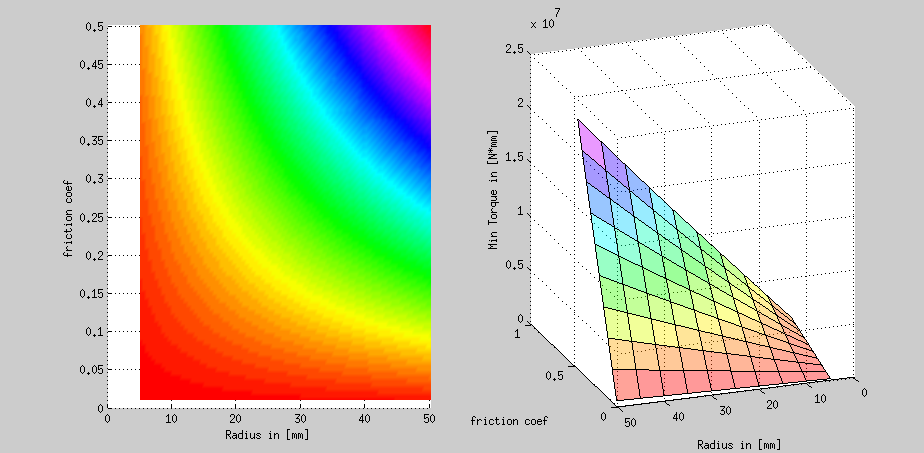
\includegraphics[width=14cm]{5.png}
\caption{Radius, friction, torque dependence}
\end{center}
\end{figure}

\newpage
%
%
%
%
%
\textbf{Title:} Determination of hypothetical model of vibration in robot mechanical structre
due to calculation of natural frequencies of system and simulating response
for specified input signal. 

\begin{figure}[!ht]
\begin{center}
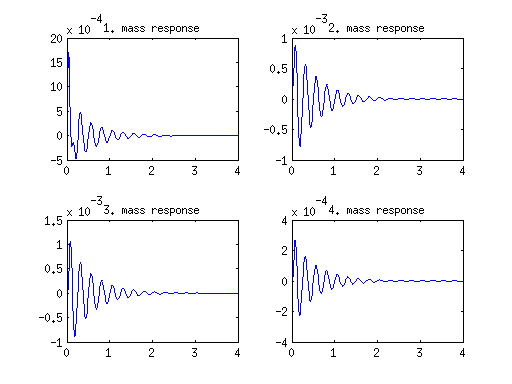
\includegraphics[width=12cm]{eksp2_01.png}
\caption{Impulse response of system forcing 1. element}
\end{center}
\end{figure}
The impulse response for input on first mass element simulate the road defect. As it can be seen
from plots, displacement is similar as in real-world. Units of displacement
on figures are meters.

\begin{figure}[!ht]
\begin{center}
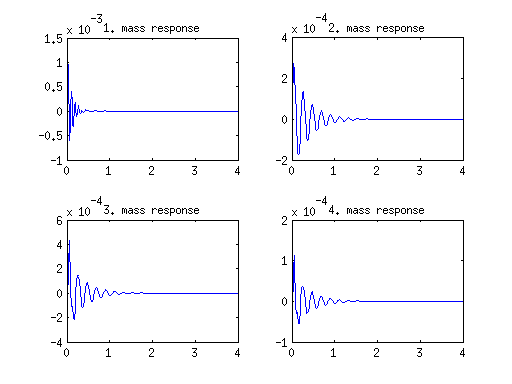
\includegraphics[width=12cm]{eksp2_02.png}
\caption{Impulse response - higher wheel elasticity coefficient}
\end{center}
\end{figure}


\begin{figure}[!ht]
\begin{center}
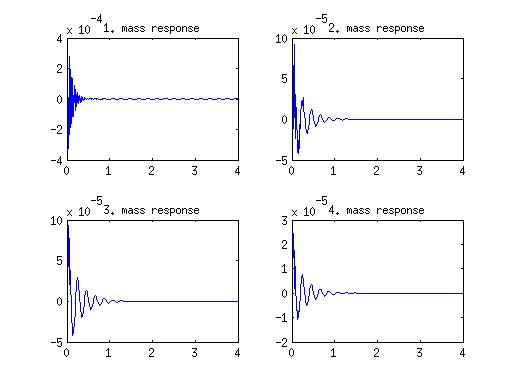
\includegraphics[width=12cm]{eksp2_03.png}
\caption{Impulse response - much higher wheel elasticity coefficient}
\end{center}
\end{figure}

\begin{figure}[!ht]
\begin{center}
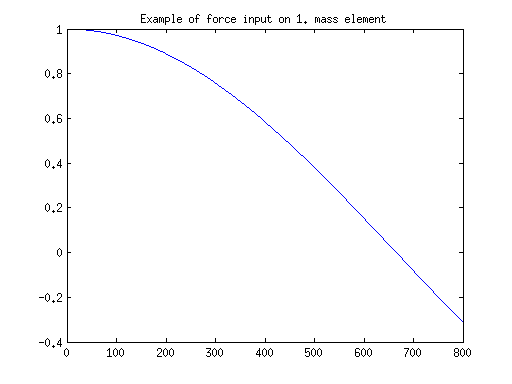
\includegraphics[width=12cm]{eksp2_04.png}
\caption{Other example of input signal}
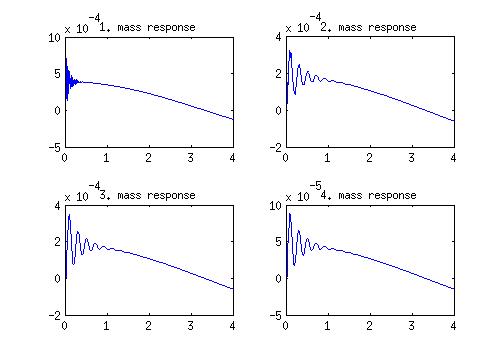
\includegraphics[width=12cm]{eksp2_05.png}
\caption{Response for given example input}
\end{center}
\end{figure}


As it can be seen, system is trying to "follow" the input signal, but at the begining
it hits high amplitude of displacement on every mass element.
\newpage
\begin{figure}[!ht]
\begin{center}
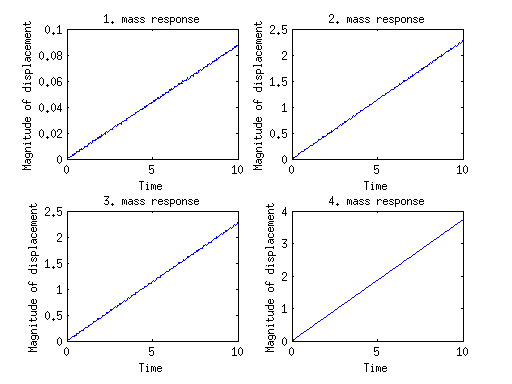
\includegraphics[width=12cm]{eksp2_06.png}
\caption{Response for natural frequencies of system sinusoidal signal}

Magnitude of displacement is growing fast in time. To protect our robot from danger
of mechanical resonance, control system and mechanical design should avoid
being close to calculated frequencies on every mass element, especially
this one with matched frequency.
\end{center}
\end{figure}

%
%
%
%
%
%
%
%

\newpage
\textbf{Title:} Analysis of sensor data in time and frequency domain. Examination of
the artifacts introduced by ADC and DAC conversion errors.
%
%
%
%
%
%
%
%\begin{equation}\label{eq:1}
%x[n]*h[n]=y[n]
%\end{equation}
%
%
%
%
%
%
%
\newpage
\section{Conclusions}
%
%
%
%
%
%
%
%
%
\section{Appendix}
\textbf{Github project repo:} 
\url{https://github.com/kfarbaniec/misk.git} \newline
To run an experiments the Matlab software is required.
Simply open the .m file with experiment you are interested 
in with Matlab and click 'Run' icon
(green triangle in Matlab editor) to run the script. \newpage
\textbf{Difficulties and design considerations} 
\par First problem in simulating vibrations was selection of spring-damper coefs values.
To choose it wisely its necessarily important to got experince and intuition.
They can
be measured and then set in model but to do it there must be some kind of 
test and measurement laboratory.
\par Generation of sample data is problematic because of 
non-deterministic real-world races. While driving, robot can possibly face
many problems not included in experiment scripts.






\section{Bibliography}
%-- z czego korzystali�my
\begin{itemize}
\item{Janusz Kowal, Podstawy Automatyki Tom I i II}
\item{Jedrzykiewisz, Teoria Sterowania Ukladow Jednowymiarowych}
\item{Jozef Giergiel, Mariusz Giergiel - Mechanika Ogolna}
\item{Fizyka, Zbigniew Kakol: http://winntbg.bg.agh.edu.pl/skrypty3/0370/fizyka.pdf}
\item{Richard G. Lyons "Wprowadzenie do cyfrowego przetwarzania sygnalow"}
\end{itemize}

\bibliographystyle{plain}
% \bibliography{bibliography.bib}

\end{document}
